%%%%%%%%%%%%%%%%%%%%%%%%%%%%%%%% 1 %%%%%%%%%%%%%%%%%%%%%%%%%%%%%%%%
\lecturetitle{\course}{Teoria dos Conjuntos}

\frame{\maketitle}


\section{Introdução}

\begin{frame}{Teoria dos Conjuntos}{Definição}

Teoria dos conjuntos é o ramo da matemática que estuda os conjuntos,
que são coleções de objetos.

\begin{block}{Características}

  \begin{itemize}
  \item É o sistema fundamental~\footnote{A teoria de conjuntos em
      questão refere-se ao sistema ZFC, ou seja, o conjunto de
      axiomas de Zermelo-Fraenkel somados ao axioma da escolha.}
    empregado na matemática atualmente;
  \item A linguagem da teoria de conjuntos pode ser usada na definição
    de quase todos os objetos matemáticos.
  \end{itemize}
  
\end{block}
  
\end{frame}

\begin{frame}{Exemplos de conjuntos}
  
  \begin{tabbing}
    \{``aba'', ``carro''\}\=  \mycomment{conjunto formado pelas
      \textit{strings} ``aba'' e ``carro''} \\
    \eumath{\{1,2,3\}} \> \mycomment{conjunto formado pelos números inteiros
      \eumath{1}, \eumath{2} e \eumath{3}}\\
    \eumath{\mathbb{N}} \> \mycomment{conjunto dos números naturais,
      \eumath{\{\alert{0},1,2,\dots\}}}\\
    \eumath{\mathbb{R}} \> \mycomment{conjunto dos números reais}\\
    \eumath{\emptyset} \> \mycomment{\alert{conjunto vazio}, possui
      nenhum elemento}\\
    $\{x|x$ é par$\}$\> \mycomment{conjunto dos números pares}\\
    $\{\{1\},2\}$ \> \mycomment{conjunto contendo $2$ e o conjunto com
    o número $1$}
  \end{tabbing}

\end{frame}

\begin{frame}{Conceitos Básicos}
    \begin{block}{Relação de Pertinência}
    \begin{tabbing}
      \eumath{o\alert{\in} A}\= \mycomment{o objeto \eumath{o} \alert{pertence} ao
        conjunto \eumath{A}, por exemplo,}\\
      \> \mycomment{o elemento \eumath{1} pertence ao conjunto
        \eumath{\{1,2,3\}}, mas \eumath{4} não.}
    \end{tabbing}
  \end{block}
  \begin{block}{Relação de Inclusão}
    \begin{tabbing}
    \eumath{A\alert{\subseteq}B}\= \mycomment{o conjunto \eumath{A} \alert{está
        contido} no conjunto \eumath{B}, ou seja,}\\ 
      \>\mycomment{\eumath{A} é formado por um \alert{subconjunto} de
        \eumath{B}, por exemplo,}\\
      \>\mycomment{\eumath{\{1,2\}} é um subconjunto de
          \eumath{\{1,2,3\}}, mas \eumath{\{3,4\}} não.}
    \end{tabbing}
  \end{block}
    
\end{frame}

\begin{frame}{Subconjunto}

Sejam os conjuntos \eumath{A} e \eumath{B}. Dizemos que 
\eumath{A} é um subconjunto de \eumath{B}, se e somente se, 
todo elemento de \eumath{A} também for elemento de \eumath{B}. 
A notação \eumath{A\subseteq B} significa que \eumath{A} é 
um subconjunto de \eumath{B}.
  
Exemplo:\\

\bigskip
\eumath{A=\{2,3,5\}}, \eumath{B=\{1,2,3,4,5,6\}} \eumath{\Rightarrow A
\subseteq B}

\end{frame}

\subsection{Quantificadores}

\begin{frame}{Quantificadores}{}

\begin{block}{Existe} 
\eumath{\exists x\in A}, afirmação sobre \eumath{x}.

\bigskip
Lê-se, existe \eumath{x} pertencente ao conjunto \eumath{A}, tal 
que a afirmação seja verdadeira. \eumath{x} é uma variável de 
referência.\\

\bigskip
Ex: \eumath{\exists x\in \mathbb{N}|} x é primo e par.
\end{block}

\begin{block}<2>{Para todo} 
\eumath{\forall x\in A}, afirmação sobre \eumath{x}.

\bigskip

Ex: \eumath{\forall x\in \mathbb{Z}}, x é ímpar ou par.
\end{block}  

\end{frame}

\begin{frame}{Combinação de quantificadores}

  \begin{enumerate}[<+-| alert@+>]
  \item Para todo x, existe um $y$ de modo que $x+y=0$,
    
    \[\forall x, \exists y | x+y=0;\]
  \item Existe um $x$, de modo que, para todo $y$, temos $x+y=0$;

    \[\exists x, \forall y | x+y=0.\]
  \end{enumerate}
  
\end{frame}

\begin{frame}{Exercícios}

  Descreva as afirmações abaixo usando os quantificadores e 
  sem se preocupar com sua veracidade.
 
  \begin{enumerate}
  \item Todo inteiro é primo.
  \item Há um inteiro que não é primo.
  \item Existe um inteiro cujo quadrado é $2$.
  \item Todos os inteiros são divisíveis por $5$.
  \item Algum inteiro é divisível por $7$.
  \item Para todo inteiro $x$, existe um inteiro $y$, de modo que 
    $xy=1$.
  \item Existem dois inteiros $x$ e $y$ de modo que $x/y=10$.
  \item Todos amam alguém alguma vez.
  \end{enumerate}

\end{frame}

\section{Operações}

\frame{\author{}\title{Operações}\date{}\maketitle}

\begin{frame}{União}
\small

\mysets
\bigskip

  \begin{columns}
    \begin{column}{.45\textwidth}
    $\erm{\{A\alert{\cup}B\deq x |x\in A\alert{\vee}x\in B\}}$

    \vspace{1cm}

    \pgfdeclarelayer{background layer}
    \pgfsetlayers{background layer,main}
    \begin{tikzpicture}
      \coordinate [label=left:$\A$] (A) at (0,0);
      \coordinate [label=right:$\B$] (B) at (1.25,0.25);
      \begin{pgfonlayer}{background layer}
        \draw[fill=setcolor] let \p1
        = ($ (B) - (A) $),
        \n{radius} = {veclen(\x1,\y1)}
        in
        (A) circle (\n{radius})
        (B) circle (\n{radius});
      \end{pgfonlayer}
    \end{tikzpicture}

    \vfill
    \vfill
    \onslide<2->{
      \centering
      \eumath{\{1,2,3,4,7\}}
    }

  \end{column}
  \begin{column}{.55\textwidth}
    $\erm{\{A\alert{\cup} B\alert{\cup}C \deq x|x\in A\alert{\vee}x \in B\alert{\vee} x\in C\}}$

    \pgfdeclarelayer{foreground layer}
    \pgfdeclarelayer{background layer}
    \pgfsetlayers{background layer,main,foreground layer}
    \begin{tikzpicture}[setcircle/.style={circle,minimum size=2.5cm,fill=setcolor,draw}]
      \begin{pgfonlayer}{foreground layer}
        \coordinate [label=above:$\A$] (A) at ($ (0,0) + .1*(rand,rand) $);
        \coordinate [label=left:$\B$] (B) at ($ (-1,-1.25) + .1*(rand,rand) $);
        \coordinate [label=right:$\C$] (C) at ($ (1,-1.25) + .1*(rand,rand) $);
      \end{pgfonlayer}
        \begin{pgfonlayer}{background layer}
          \filldraw [setcircle]  (A) circle (1.2cm);
          \filldraw [setcircle]  (B) circle (1.2cm);
          \filldraw [setcircle]  (C) circle (1.2cm);
        \end{pgfonlayer}
        \begin{pgfonlayer}{foreground layer}
          \draw []  (A) circle (1.2cm);
          \draw []  (B) circle (1.2cm);
          \draw []  (C) circle (1.2cm);
        \end{pgfonlayer}
      
      \end{tikzpicture}
      
      \vfill
    
      \onslide<3>{
        \centering
        \eumath{\{1,2,3,4,5,7,10\}}
      }
  \end{column}
\end{columns}



\end{frame}

\begin{frame}{Intersecção}

\small
\mysets\bigskip

  \begin{columns}
    \begin{column}{.425\textwidth}
      $\erm{\{A\alert{\cap}B\deq x |x\in A\alert{\wedge}x\in B\}}$
      
      \begin{center}
      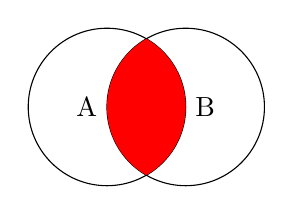
\begin{tikzpicture}
        \draw[] (1,0) circle (1cm) node[anchor=west] {B} ;
        \draw[clip] (0,0) circle (1cm) node[anchor=east] {A} ;
        \fill[red] (1,0) circle (1cm);
      \end{tikzpicture}
    \end{center}
    
    \vfill
    \onslide<2->{
      \begin{center}
        \eumath{\{2,4\}}
      \end{center}
    }
  
\end{column}
  \begin{column}{.575\textwidth}
    $\erm{\{A\alert{\cap}B\alert{\cap}C\deq x|x\in A\alert{\wedge}x\in B\alert{\wedge}x\in C\}}$
    
    \begin{center}
    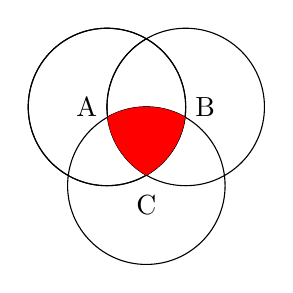
\begin{tikzpicture}
      \draw[] (0,0) circle (1cm) node[anchor=east] {A};
      \draw[] (1,0) circle (1cm) node[anchor=west] {B};
      \draw[] (.5,-1) circle (1cm) node[anchor=north] {C};
      \begin{scope}
        \draw[clip] (0,0) circle (1cm);
        \draw[clip] (1,0) circle (1cm);
        \draw[clip] (.5,-1) circle (1cm);
        \fill[red] (0,0) circle (1cm);
        \fill[red] (1,0) circle (1cm);

      \end{scope}
    \end{tikzpicture}
  \end{center}

\vfill
\onslide<3>{
\begin{center}
\eumath{\{4\}}
\end{center}
}
\end{column}
\end{columns}
\end{frame}

\begin{frame}{Diferença}

\eumath{\{A\backslash B \deq x|x\in A \wedge x \notin B\}}
    \begin{center}
    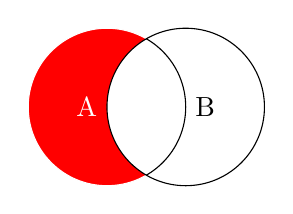
\begin{tikzpicture}
      \begin{scope}
        \fill[red] (0,0) circle (1cm);
        \draw[white] (0,0) circle (1cm) node[anchor=east] {A} ;
      \end{scope}
      \fill[white] (1,0) circle (1cm);
      \draw[clip] (1,0) circle (1cm) node[anchor=west] {B} ;
      \draw[] (0,0) circle (1cm) node[anchor=east] {} ;
  \end{tikzpicture}
  \end{center}

\onslide<2>

\[\setA,\setB\]
\[A\backslash B= \{1\}\]

\end{frame}

\begin{frame}{Diferença simétrica}
  \[ \{A\Delta B \deq (A\cup B)\backslash (A\cap B)\}\]

     \begin{center}
     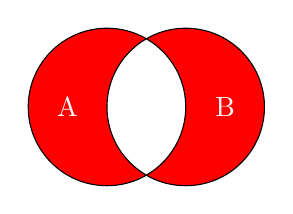
\begin{tikzpicture}
       \filldraw[even odd rule,red,draw=black] (6,0) circle (1cm)  (7,0) circle (1cm);
       \node[white] at (5.5,0) {A};
       \node[white] at (7.5,0) {B};
     \end{tikzpicture}
   \end{center}

\onslide<2>

\[\setA,\setB\]
\[A\Delta B= \{1,3,7\}\]

\end{frame}

%%%%%%%%%%%%%%%%%%%%%%%%%%%%%%%% AULA 2
%%%%%%%%%%%%%%%%%%%%%%%%%%%%%%%% ################################

\begin{frame}{Produto Cartesiano}
  
  \eumath{\tuple{x,y} |x\in A \wedge y \in B }
  
  Ex: \eumath{\setA, \setB}
  \begin{tabbing}
    \eumath{A\times B =}\=\eumath{\{ \tuple{1,2},\tuple{1,3},\tuple{1,4},\tuple{1,7},}\\
    \>\eumath{\tuple{2,2},\tuple{2,3},\tuple{2,4},\tuple{2,7},}\\
    \>\eumath{\tuple{4,2},\tuple{4,3},\tuple{4,4},\tuple{4,7}\}}
  \end{tabbing}

  \pgfdeclarelayer{foreground layer}
  \pgfdeclarelayer{background layer}
  \pgfsetlayers{background layer,main,foreground layer}
\begin{center}
  \begin{tikzpicture}[every path/.style={draw},
    every ellipse/.style={minimum width=1cm,draw}]
    
    \begin{pgfonlayer}{foreground layer}
      \node (a1) {\eumath{1}};
      \node (a2) [below of=a1] {\eumath{2}};
      \node (a4) [below of=a2] {\eumath{4}};
      \node (b2) [right of=a1,yshift=.5cm,xshift=2cm] {\eumath{2}};
      \node (b3) [below of=b2] {\eumath{3}};
      \node (b4) [below of=b3] {\eumath{4}};
      \node (b7) [below of=b4] {\eumath{7}};
    \end{pgfonlayer}
  
  \begin{pgfonlayer}{background layer}
      \node[fill=yellow,ellipse,minimum width=1cm,minimum
      height=3cm,draw] at (a2) [below of=a1] {};
      \node[fill=blue!40,ellipse,minimum height=4cm,minimum width=1cm,draw] at (b3.south) {};
    \end{pgfonlayer}
  
    \begin{pgfonlayer}{foreground layer}
    \path (a1) -- (b2) -- (a2) -- (b3) -- (a4) -- (b4) -- (a2) -- (b7)
    -- (a4) -- (b2);
    \path (a1) -- (b3);
    \path (a1) -- (b4);
    \path (a1) -- (b7);
  \end{pgfonlayer}
  
  \end{tikzpicture}
\end{center}

\end{frame}


\begin{frame}{Exercício}

  Para os conjuntos $A=\{1,2,3,4,5\}$ e $B=\{4,5,6,7\}$, determine:

  \begin{enumerate}
  \item $A\cup B$
  \item $A\cap B$
  \item $A\backslash B$
  \item $B\backslash A$
  \item $A\Delta B$
  \item $B\Delta A$
  \item $A\times B$
  \item $B\times A$
  \end{enumerate}

\end{frame}

\begin{frame}{$+$Exercício}
  
  Suponha o conjunto universo $S=\{0,1,2,3,4,5,6,7,8,9\}$, bem como 
  os seguintes conjuntos:
  \[A=\{2,4,5,6,8\}\]
  \[B=\{1,4,5,9\}\]
  \[C=\{x|x\in \mathbb{Z} \wedge 2\leq x<5\}\]
  \noindent Então determine:
  \bigskip
  \begin{enumerate}
    \begin{minipage}{.25\textwidth}
    \item $A\cup B$
    \item $A\cap B$
    \item $A\cap C$
    \item $B\cup C$
    \item $A\backslash B$
    \item $\neg A$
    \end{minipage}
    \begin{minipage}{.25\textwidth}
    \item $A\cap\neg A$
    \item $\neg (A\cap B)$
    \item $C\backslash B$
    \item $(C\cap B) \cup \neg A$
    \item $\neg (B\backslash A)\cap (A\backslash B)$
    \end{minipage}
  \end{enumerate}
  
\end{frame}

\begin{frame}{$++$Exercícios}

\begin{enumerate}
  \item Sejam $A$ e $B$ conjuntos e suponha que 
  $A\times B=\{\tuple{1,2},\tuple{1,3},\tuple{2,2},\tuple{2,3}\}$.\\
  Encontre $A\cup B$, $A\cap B$, $A\backslash B$.
\item Suponha que $A$ e $B$ sejam conjuntos finitos. Dado que $|A|=10$, 
 $|A\cup B|=15$ e $|A\cap B|=3$, determine $|B|$.
\end{enumerate}

\end{frame}

